This section outlines the various components of the system and how they interact with one and another. The detailed architecture is described in figure \ref{sec:architecture:fig:O-Architecture}.

\begin{figure*}[ht]
\label{sec:architecture:fig:O-Architecture}
\caption{Original Architecture Design}
\centering
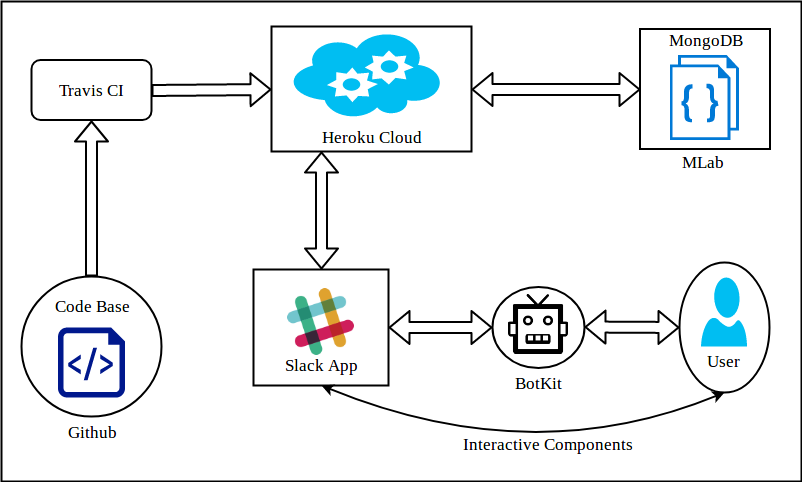
\includegraphics[width=\textwidth]{O-Architecture.png}
\end{figure*}

Broadly speaking, we can divide the architecture in three main components. The slack app, the heroku cloud and the mongoDB database. This separation of concerns is a major advantage since database is independently hosted on mlab server and can be accessed from anywhere with valid autho- rization credentials. The heroku cloud hosts the logic of the slack app, which communicates with the user. We have also implemented the continuous deployment, continuous inte- gration pipeline with Travis CI, which directly pushes the code to heroku cloud once the build passes (also indicated in the readme section of the repository). We have written test cases which acts as a sanity check for any commit made to the master branch, before deployment so as to not push broken code on the production server at heroku. Following is the detailed description of each component of our archi- tecture.

% \paragraph{
%%% Local Variables:
%%% mode: latex
%%% TeX-master: "../../../main"
%%% End:
